% ===============================================================
%  جلسه هفتم
% ===============================================================
\chapter{متغیرهای تصادفی پیوسته، \lr{CDF} و \lr{PDF}}

\section[متغیرهای تصادفی پیوسته]{متغیرهای تصادفی پیوسته {\large\lr{(Continuous R.V.s)}}}

پیش‌تر دیدیم که مدل‌سازی تصادفی یک واقعه، معادل با تعریف یک فضای احتمال به صورت $(\Omega,\F,P)$ است. این تعاریف، در مورد خود یک متغیر تصادفی نیز برقرار هستند: می‌توانیم به جای فضای پیچیده اولیه، مجموعه مقادیر خود متغیر تصادفی را به عنوان فضای نمونه در نظر بگیریم. برای مثال، در مورد یک \textcolor{red!70!black}{متغیر تصادفی گسسته}، $\Omega$ فضای شمارای مقادیری است که متغیر می‌تواند بگیرد:
\begin{itemize}
\item برای متغیر تصادفی برنولی داریم $\Omega=\{0,1\}$،
\item در مورد یک توزیع دوجمله‌ای داریم $\Omega=\{0,1,\ldots,n\}$،
\item و برای متغیر تصادفی با توزیع پواسون خواهیم داشت $\Omega=\N_{\ge0}$.
\end{itemize}
در تمام موارد بالا، برای فضای وقایع (یعنی $\F$)، قرار می‌دهیم $\F=2^\Omega$.

\subsection{مشکل فضای ناشمارا}
در مورد متغیرهای تصادفی پیوسته (\lr{Continuous R.V.s}) معمولاً داریم $\Omega=\R$. در این حالات معمولاً (البته نه همیشه!) احتمال بروز تک‌مقدارها صفر هستند. برای مثال، اگر $X$ یک متغیر تصادفی کاملاً پیوسته باشد، خواهیم داشت:
\[
\Prob(X=1.2)=\Prob(X=-\sqrt2)=\cdots=0 .
\]

\begin{question}[اما احتمال بازه‌ها چطور؟ آیا می‌توان مطابق رابطه زیر نتیجه گرفت؟ چرا این رابطه اشتباه است؟]
\[
\Prob(X\in A)=\sum_{x\in A}\Prob(X=x),\qquad\forall A\in\F .
\]
\begin{answer}
این رابطه اشتباه است زیرا اصل جمع‌پذیری کولموگروف فقط برای اجتماع‌های \textbf{شمارا} برقرار است، در حالی که یک بازه مانند $[0,1]$ اجتماع \textbf{ناشمارا}یی از نقاط است. اگر این رابطه درست بود، چون همه $\Prob(X=x)=0$ هستند، نتیجه می‌گرفتیم $\Prob(X\in\R)=\sum_{x\in\R}0=0$، که با $\Prob(\Omega)=1$ در تناقض است. پس احتمال یک بازه را نمی‌توان از احتمال نقاط آن به دست آورد؛ بلکه باید مستقیماً برای مجموعه‌ها (بازه‌ها) احتمال تعریف کنیم.
\end{answer}
\end{question}

همان‌طور که ملاحظه کردید، در مورد متغیرهای تصادفی پیوسته می‌بایست به صورت مجزا برای زیرمجموعه‌های $\R$ احتمال تعریف کنیم (نمی‌توانیم مستقیماً از اصول کولموگروف استفاده کرده و احتمالشان را به صورت جمع احتمال اعضای آنان بنویسیم؛ به دلیل \textbf{ناشمارا} (\lr{uncountable}) بودن).

اما این سؤال مطرح می‌شود که برای کدام زیرمجموعه‌های $\R$ می‌توانیم احتمال تعریف کنیم\ldots\ بهتر است سراغ تمام زیرمجموعه‌های موجود در $2^\R$ نرویم! (برای مطالعه بیشتر به سراغ عواقب ناخواسته \textbf{اصل انتخاب} (\lr{Axiom of Choice}) در مجموعه‌ها، و همچنین \lr{Banach--Tarski paradox} بروید.)

\begin{note}
\notetitle \textbf{چرا همه زیرمجموعه‌ها نه؟} با پذیرش اصل انتخاب می‌توان زیرمجموعه‌هایی «بسیار عجیب» از $\R$ ساخت (مانند مجموعه ویتالی) که به هیچ وجه نمی‌توان به آن‌ها «طول» یا «احتمال» سازگار با اصول کولموگروف نسبت داد. پارادوکس باناخ--تارسکی حتی نشان می‌دهد که یک کره را می‌توان به چند تکه (غیراندازه‌پذیر) تقسیم کرد و با جابه‌جایی و چرخش آن‌ها دو کره هم‌اندازه کره اول ساخت! پس باید خود را به زیرمجموعه‌های «خوش‌رفتار» محدود کنیم.
\end{note}

\subsection{مجموعه‌ها و میدان سیگمای بورل \lr{(Borel Sets and Borel $\sigma$-Field)}}

به جای تمامی زیرمجموعه‌های $\R$، فقط سراغ زیرمجموعه‌های \textcolor{red!70!black}{معقول و زیبای} آن می‌رویم! و صرفاً برای آنان احتمال تعریف می‌کنیم.

\begin{definition}[مجموعه بورل]
زیرمجموعه‌های معقول و زیبا (\lr{nice}) روی $\R$ را به صورت زیر تعریف می‌کنیم:
\[
\bigcup_{i=1}^{\infty}I_i\subseteq\R,\qquad \text{where } I_i\text{s are intervals},
\]
که در اینجا، هر $I_i$ یک بازه کاملاً دلخواه (مانند $(-\infty,4.7]$، یا $(3,4.2)$، یا $[1,1]$، و غیره) روی $\R$ است. همچنین دنباله $\{I_1,I_2,\ldots\}$ می‌تواند محدود، یا نامحدود (ولی شمارا) باشد. به هر زیرمجموعه‌ای از $\R$ که بتواند به شکل بالا (یا متمم آن، و به‌طور کلی با تکرار شمارای این اعمال) نوشته شود یک \lr{Borel set} می‌گوییم.
\end{definition}

\begin{theorem}
مجموعه تمام \lr{Borel set}های روی $\R$ تشکیل یک \lr{$\sigma$-Field} می‌دهند. به آن \textbf{میدان سیگمای بورل} گفته و با $\mathcal{B}(\R)$ نشان می‌دهیم. (به طور دقیق، $\mathcal{B}(\R)$ کوچک‌ترین میدان سیگمایی است که شامل همه بازه‌هاست.)
\end{theorem}

تقریباً هر مجموعه‌ای که در عمل با آن سر و کار داریم بورل است: بازه‌ها، نقاط تکی، مجموعه‌های شمارا (مثل اعداد گویا)، اجتماع و اشتراک شمارای بازه‌ها و \ldots

در این صورت، می‌توانیم با خیال راحت فضای وقایع قابل اندازه‌گیری (یعنی $\F$) را به صورت یک \lr{Borel $\sigma$-Field} روی $\R$ در نظر بگیریم.

\subsection{کافی بودن احتمال بازه‌ها}
در این صورت، برای تعریف احتمال برای تمامی اعضای $\F$ (یعنی یک واقعه یا \lr{Event})، کافی است احتمال را برای هر بازه (مثلاً $(a,b]$) به ازای تمامی مقادیر $a,b\in\R$ با شرط $b\ge a$ تعریف کرده باشیم. سپس با استفاده از قوانین کولموگروف احتمال تمامی وقایع به صورت خودکار تعریف می‌شود.

\begin{question}[چرا؟]
\begin{answer}
هر مجموعه بورل از بازه‌ها با تعداد شمارایی عمل اجتماع، اشتراک و متمم ساخته می‌شود. اصول کولموگروف دقیقاً به ما می‌گویند احتمال تحت این اعمال چگونه رفتار می‌کند:
\begin{itemize}
\item احتمال اجتماع شمارای بازه‌های ناسازگار = جمع احتمال بازه‌ها (جمع‌پذیری شمارا)؛ هر اجتماع شمارا از بازه‌ها را هم می‌توان به اجتماع شمارای بازه‌های ناسازگار تبدیل کرد.
\item احتمال متمم = یک منهای احتمال.
\item احتمال یک نقطه هم از بازه‌ها به دست می‌آید: $\{a\}=\bigcap_{n}(a-\frac1n,a]$ و با پیوستگی احتمال $\Prob(X=a)=\lim_n\Prob(a-\frac1n<X\le a)$.
\end{itemize}
بنابراین احتمال هر مجموعه بورل به‌طور یکتا از احتمال بازه‌ها تعیین می‌شود. (اثبات کامل این گزاره ــ «قضیه گسترش کاراتئودوری» ــ در درس نظریه اندازه دیده می‌شود.)
\end{answer}
\end{question}

پس به یک تابع مانند $P(a,b)$ نیاز داریم که به ازای $a,b$ ورودی احتمال بازه $(a,b]$ را بازگرداند. اما می‌توان به راحتی این تابع را به یک متغیر ورودی کاهش داد. \textbf{چگونه؟} چون $(-\infty,b]=(-\infty,a]\cup(a,b]$ و این دو ناسازگارند:
\[
P\big((a,b]\big)=P\big((-\infty,b]\big)-P\big((-\infty,a]\big).
\]
پس کافی است تابع یک‌متغیره $x\mapsto P((-\infty,x])$ را بدانیم. این همان تابع توزیع انباشته است.

\section{تابع توزیع انباشته \lr{(Cumulative Distribution Function)}}

\begin{definition}[تابع توزیع انباشته \lr{(CDF)}]
تابع توزیع انباشته (\lr{CDF}) متغیر تصادفی $X$ را به صورت زیر تعریف می‌کنیم:
\[
F_X(x)=\Prob\{X\le x\}.
\]
لذا $F_X$ یک تابع از اعداد (مثلاً اعداد حقیقی) به بازه بسته $[0,1]$ است.
\end{definition}

\begin{warning}
\warntitle \textbf{اشتباه رایج:} دقت کنید که در این رابطه، $X$ بیان‌گر منتسب بودن $F_X$ به یک متغیر تصادفی خاص است. ولی $x$ یک عدد (مثلاً یک عدد حقیقی) و در اینجا صرفاً یک متغیر کمکی (در اصطلاح \lr{dummy variable}) است. مثلاً $F_X(2)=\Prob(X\le2)$ و $F_Y(2)=\Prob(Y\le2)$ دو عدد متفاوت‌اند.
\end{warning}

\begin{theorem}[ویژگی‌های \lr{CDF}]
برای هر متغیر تصادفی $X$:
\begin{enumerate}
\item تابع $F_X$ \textbf{صعودی} (غیرنزولی) است، ولی لزوماً \textbf{اکیداً صعودی} نیست.
\item مقادیر حدی:
$\ F_X(-\infty)=\lim_{x\to-\infty}F_X(x)=0,\qquad F_X(+\infty)=\lim_{x\to+\infty}F_X(x)=1 .$
\item $F_X$ از راست پیوسته است: $\lim_{h\to0^+}F_X(x+h)=F_X(x)$.
\item $\Prob(a<X\le b)=F_X(b)-F_X(a)$ و $\Prob(X=a)=F_X(a)-F_X(a^-)$ (اندازه پرش در نقطه $a$).
\end{enumerate}
\end{theorem}
\begin{proof}
(۱) اگر $x<y$ آنگاه $\{X\le x\}\subseteq\{X\le y\}$ و طبق یکنوایی احتمال، $F_X(x)\le F_X(y)$. اما اکیداً صعودی نیست چون اگر $X$ هیچ مقداری در بازه $(x,y]$ نگیرد، $\Prob(x<X\le y)=0$ و $F_X$ روی این بازه ثابت می‌ماند (مانند نواحی افقی در \lr{CDF} یک متغیر گسسته، یا بیرون بازه $[a,b]$ در توزیع یکنواخت).
(۲) وقتی $x\to-\infty$، رویدادهای $\{X\le x\}$ به $\varnothing$ و وقتی $x\to+\infty$ به $\Omega$ میل می‌کنند؛ با پیوستگی احتمال حدود ۰ و ۱ به دست می‌آیند.
(۳) و (۴) نیز از پیوستگی احتمال و تعریف به دست می‌آیند.
\end{proof}

\begin{figure}[H]
\centering
\begin{tikzpicture}
\begin{axis}[width=5.2cm,height=4.4cm,xmin=-1,xmax=3.5,ymin=-0.05,ymax=1.15,ytick={0,0.25,0.75,1},yticklabels={$0$,$\frac14$,$\frac34$,$1$},xtick={0,1,2,3},title={\small گسسته (پله‌ای)},axis lines=middle]
\addplot[very thick,domain=-1:0] {0};
\addplot[very thick,domain=0:1] {0.25};
\addplot[very thick,domain=1:2] {0.75};
\addplot[very thick,domain=2:3.5] {1};
\addplot[only marks,mark=*] coordinates {(0,0.25) (1,0.75) (2,1)};
\addplot[only marks,mark=o,fill=white] coordinates {(0,0) (1,0.25) (2,0.75)};
\end{axis}
\end{tikzpicture}
\begin{tikzpicture}
\begin{axis}[width=5.2cm,height=4.4cm,xmin=0,xmax=4,ymin=0,ymax=1.1,xtick={1,3},xticklabels={$a$,$b$},title={\small یکنواخت},axis lines=left]
\addplot[very thick,blue] coordinates {(0,0) (1,0) (3,1) (4,1)};
\end{axis}
\end{tikzpicture}
\begin{tikzpicture}
\begin{axis}[width=5.2cm,height=4.4cm,xmin=-3,xmax=3,ymin=0,ymax=1.1,title={\small گاوسی (هموار)},axis lines=left,samples=80]
\addplot[very thick,domain=-3:3] {1/(1+exp(-1.7*x))};
\end{axis}
\end{tikzpicture}
\caption{سه نمونه \lr{CDF}: سمت راست مربوط به تعداد شیرها در دو پرتاب سکه (پرش‌هایی به اندازه $\frac14,\frac12,\frac14$)، وسط توزیع یکنواخت روی $[a,b]$، و چپ یک \lr{CDF} هموار.}
\end{figure}

\begin{note}
\notetitle \lr{CDF} برای \emph{همه} متغیرهای تصادفی (گسسته، پیوسته یا ترکیبی) تعریف می‌شود و توزیع را به‌طور کامل مشخص می‌کند. برای متغیر گسسته، \lr{CDF} پله‌ای است و ارتفاع هر پله برابر \lr{PMF} در آن نقطه است.
\end{note}

\section{تابع چگالی احتمال \lr{(Probability Density Function)}}

\subsection{مفهوم}
کار کردن با تابع توزیع انباشته (\lr{CDF}) مقداری سخت است:
\begin{itemize}
\item شهود بالایی نسبت به آن نداریم.
\item اطلاعات محلی (\lr{localized}) مناسبی از نواحی مختلف فضا به دست نمی‌دهد (مقدار $F_X(x)$ همه جرم احتمال در سمت چپ $x$ را با هم جمع می‌کند).
\end{itemize}
برای حل این مشکل، از تابع چگالی احتمال (\lr{PDF}) استفاده خواهد شد:

\begin{definition}[تابع چگالی احتمال]
\[
f_X(x)=\lim_{h\to0^+}\frac{P\big(x<X\le x+h\big)}{h}=\frac{\dd F_X(x)}{\dd x}.
\]
\end{definition}
عبارت وسط \textbf{مفهوم چگالی دارد}: احتمال (جرم) واقع در یک بازه کوچک تقسیم بر طول آن بازه ــ دقیقاً مانند چگالی جرم در فیزیک (جرم بر واحد طول). به بیان دیگر، برای $h$ کوچک:
\[
P(x<X\le x+h)\approx f_X(x)\,h .
\]

\subsection{خواص و مقایسه با سایر توابع}
تابع چگالی احتمال (\lr{PDF}):
\begin{itemize}
\item $f_X(x)$ همواره نامنفی است ($f_X\ge0$)؛ زیرا مشتق یک تابع صعودی است.
\item $f_X(x)$ \textbf{لزوماً بین ۰ و ۱ نیست}. حتی ممکن است گاهی بی‌نهایت شود (\textcolor{red!70!black}{دقت کنید که $f_X$ به خودی خود معنای احتمال ندارد}). مثال: برای $X\sim\mathrm{Uniform}(0,0.1)$ داریم $f_X=10$ روی بازه.
\item شرط بهنجارش (\lr{Normalization criteria}):
\[
\int_{-\infty}^{+\infty}f_X(x)\dd x=F_X(+\infty)-F_X(-\infty)=1 .
\]
\end{itemize}

\begin{summarybox}[مقایسه توابع \lr{CDF}، \lr{PDF}، \lr{PMF} و اندازه احتمال $P$]
\begin{itemize}
\item \textbf{اندازه احتمال $P$} (\lr{Probability Measure or Law}): عضو سوم فضای احتمال $(\Omega,\F,P)$، که به هر رویداد در $\F$ عددی در بازه $[0,1]$ نسبت می‌دهد که می‌بایست قوانین کولموگروف را رعایت نماید.
\item \textbf{تابع توزیع انباشته \lr{CDF}:} در نقطه $x\in R$ به معنای $P(X\le x)$ خواهد بود. \lr{CDF} معنای احتمال دارد و بین $[0,1]$ خواهد بود. همچنین تابعی صعودی است که در $-\infty$ برابر با صفر، و در $+\infty$ برابر با یک است.
\item \textbf{تابع چگالی احتمال \lr{PDF}:} مشتق تابع \lr{CDF}، که همواره نامنفی و عددی در $\R_{\ge0}$ خواهد بود. \lr{PDF} مفهوم احتمال ندارد، و صرفاً انتگرال آن معنای احتمال می‌دهد:
\[
\boxed{\ P\big(a<X\le b\big)=\int_a^bf_X(x)\dd x=F_X(b)-F_X(a)\ }
\]
\item \textbf{تابع جرم احتمال \lr{PMF}:} زمانی که $\Omega$ مجموعه‌ای محدود (یا شمارا) باشد، برای $\Omega=\{\omega_1,\ldots,\omega_N\}$ به صورت $p(\omega_i)=P(\{\omega_i\})$ تعریف می‌شود. لذا معنای احتمال دارد و همواره بین ۰ و ۱ است. همچنین، جمع \lr{PMF} روی کل $\Omega$ برابر با ۱ می‌شود.
\end{itemize}
\end{summarybox}

\subsection{مفهوم گرافیکی}
احتمال اینکه $X$ در بازه $(a,b]$ بیفتد، برابر \textbf{مساحت زیر منحنی} \lr{PDF} بین $a$ و $b$ است:

\begin{center}
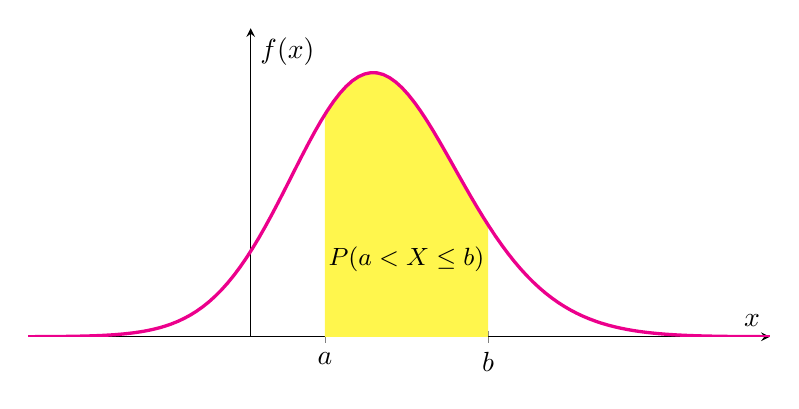
\begin{tikzpicture}
\begin{axis}[width=11cm,height=5.5cm,axis lines=middle,xmin=-3,xmax=7,ymin=0,ymax=0.32,xtick={1,3.2},xticklabels={$a$,$b$},ytick=\empty,xlabel={$x$},ylabel={$f(x)$},samples=120,domain=-3:7]
\addplot[fill=yellow!70,draw=none,domain=1:3.2] {0.12*exp(-0.5*((x-2)/1.3)^2)+0.16*exp(-0.5*((x-1.5)/1.0)^2)} \closedcycle;
\addplot[very thick,magenta] {0.12*exp(-0.5*((x-2)/1.3)^2)+0.16*exp(-0.5*((x-1.5)/1.0)^2)};
\node at (axis cs:2.1,0.08) {\small $P(a<X\le b)$};
\end{axis}
\end{tikzpicture}
\end{center}

\begin{note}
\notetitle برای متغیر پیوسته $P(X=a)=0$، پس $P(a<X\le b)=P(a\le X\le b)=P(a<X<b)$؛ یعنی باز یا بسته بودن انتهای بازه مهم نیست. این برای متغیرهای گسسته \emph{درست نیست}.
\end{note}

\section{متغیرهای تصادفی پیوسته معروف}

\subsection{توزیع یکنواخت \lr{(Uniform Distribution)}}
متغیر تصادفی یکنواخت، دارای بیشترین آنتروپی (تصادفی بودن) بین تمامی متغیرهای تصادفی با $\Omega=[a,b]$ است؛ یعنی وقتی فقط می‌دانیم مقدار در $[a,b]$ است و هیچ اطلاع دیگری نداریم، «بی‌طرفانه‌ترین» مدل است. این متغیر تصادفی دارای دو پارامتر آزاد $a$ و $b$ ($b>a$) است.

\begin{definition}[توزیع یکنواخت]
برای $X\sim\mathrm{Uniform}(a,b)$:
\[
f_X(x)=\begin{cases}\dfrac{1}{b-a} & a\le x\le b\\[2mm] 0 & \text{o.w.}\end{cases}
\qquad\qquad
F_X(x)=\begin{cases}0 & x<a\\ \dfrac{x-a}{b-a} & a\le x\le b\\ 1 & x>b\end{cases}
\]
\end{definition}
احتمال هر زیربازه $[c,d]\subseteq[a,b]$ متناسب با طول آن است: $P(c\le X\le d)=\frac{d-c}{b-a}$.

\begin{center}
\begin{tikzpicture}
\begin{axis}[width=8cm,height=4.5cm,axis lines=left,xmin=0,xmax=5,ymin=0,ymax=0.7,xtick={1,4},xticklabels={$a$,$b$},ytick={0.3333},yticklabels={$\frac1{b-a}$},xlabel={$x$},ylabel={$f(x)$}]
\addplot[very thick,blue] coordinates {(0,0) (1,0)};
\addplot[very thick,blue] coordinates {(1,0.3333) (4,0.3333)};
\addplot[very thick,blue] coordinates {(4,0) (5,0)};
\addplot[dashed,blue] coordinates {(1,0) (1,0.3333)};
\addplot[dashed,blue] coordinates {(4,0) (4,0.3333)};
\end{axis}
\end{tikzpicture}
\end{center}

\subsection{توزیع نمایی \lr{(Exponential Distribution)}}
توزیع نمایی (\lr{Exponential}) دارای یک پارامتر آزاد به صورت $\lambda\in\R_{>0}$ است.
\begin{definition}[توزیع نمایی]
برای $X\sim\mathrm{exponential}(\lambda)$:
\[
f_X(x)=\begin{cases}\lambda e^{-\lambda x} & x\ge0\\ 0 & x<0\end{cases}
\qquad\qquad
F_X(x)=\begin{cases}1-e^{-\lambda x} & x\ge0\\ 0 & x<0\end{cases}
\]
\end{definition}
محاسبه \lr{CDF}: برای $x\ge0$، $F_X(x)=\int_0^x\lambda e^{-\lambda t}\dd t=\big[-e^{-\lambda t}\big]_0^x=1-e^{-\lambda x}$.

این توزیع معمولاً برای مدل‌سازی \textbf{زمان وقوع} یک رخداد \textbf{بی‌حافظه} مورد استفاده قرار می‌گیرد (مثلاً زمان تا خرابی یک قطعه الکترونیکی، یا زمان بین دو تماس متوالی در فرایند پواسون).

\begin{center}
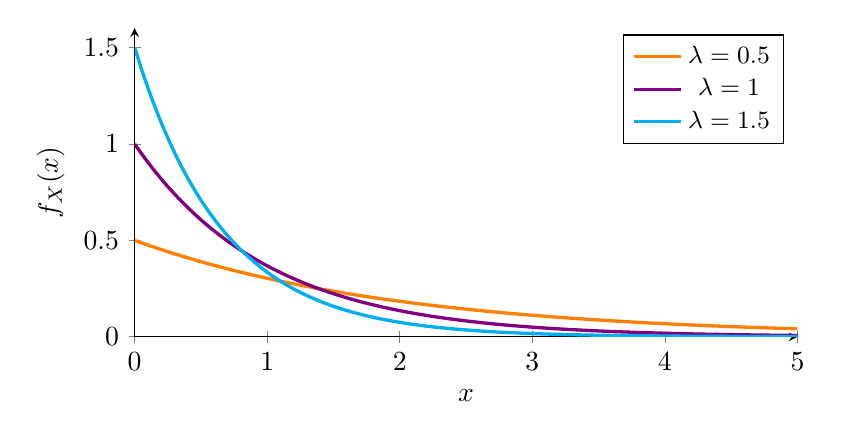
\begin{tikzpicture}
\begin{axis}[width=10cm,height=5.5cm,axis lines=left,xmin=0,xmax=5,ymin=0,ymax=1.6,xlabel={$x$},ylabel={$f_X(x)$},samples=100,domain=0:5,legend style={font=\small}]
\addplot[orange,very thick] {0.5*exp(-0.5*x)}; \addlegendentry{$\lambda=0.5$}
\addplot[violet,very thick] {exp(-x)}; \addlegendentry{$\lambda=1$}
\addplot[cyan,very thick] {1.5*exp(-1.5*x)}; \addlegendentry{$\lambda=1.5$}
\end{axis}
\end{tikzpicture}
\end{center}

\begin{theorem}[خاصیت بی‌حافظگی]
اگر $X\sim\mathrm{exponential}(\lambda)$، آنگاه برای هر $s,t\ge0$:
\[
P(X>s+t\given X>s)=P(X>t).
\]
\end{theorem}
\begin{proof}
$P(X>x)=1-F_X(x)=e^{-\lambda x}$. پس
\[
\begin{aligned}
P(X>s+t\given X>s)&=\frac{P(X>s+t,\ X>s)}{P(X>s)}=\frac{P(X>s+t)}{P(X>s)}\\
&=\frac{e^{-\lambda(s+t)}}{e^{-\lambda s}}=e^{-\lambda t}=P(X>t).
\end{aligned}
\]
\end{proof}
تعبیر: اگر یک لامپ با طول عمر نمایی تا لحظه $s$ سالم مانده باشد، احتمال اینکه $t$ واحد دیگر هم سالم بماند دقیقاً مثل یک لامپ نو است؛ لامپ «پیر نمی‌شود».

\subsection{توزیع گاوسی یا نرمال \lr{(Gaussian or Normal Distribution)}}
یکی از پرکاربردترین توزیع‌های آماری، توزیع احتمال گاوسی یا نرمال است. توزیع گاوسی $\mathcal N(\mu,\sigma^2)$ با دو پارامتر آزاد مشخص می‌شود:
\begin{itemize}
\item \textbf{میانگین} (\lr{mean}) $\mu\in\R$، و \textbf{واریانس} (\lr{variance}) $\sigma^2\in\R_{\ge0}$.
\item به خود مقدار $\sigma\in\R_{\ge0}$ \textbf{انحراف معیار} (\lr{standard deviation}) اطلاق می‌گردد.
\end{itemize}

\begin{definition}[توزیع گاوسی]
برای $X\sim\mathcal N(\mu,\sigma^2)$:
\[
f_X(x)=\frac{1}{\sqrt{2\pi}\,\sigma}e^{-\frac{(x-\mu)^2}{2\sigma^2}} .
\]
\end{definition}

\begin{center}
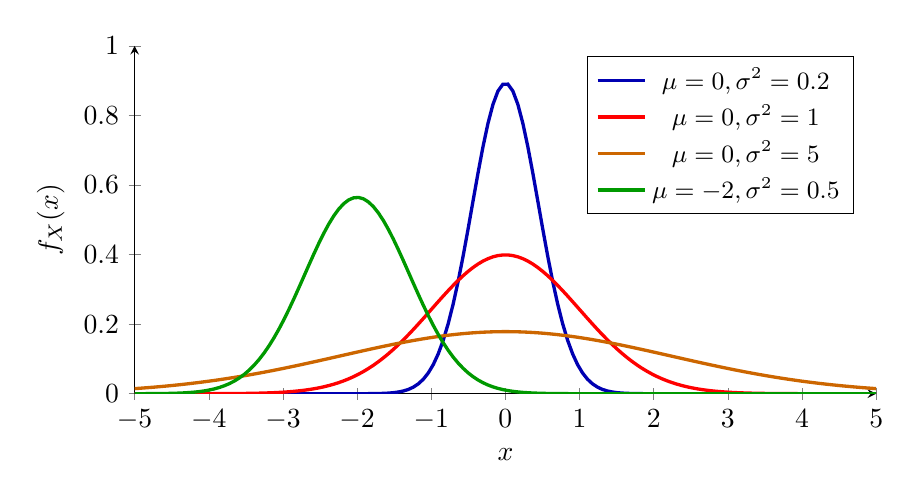
\begin{tikzpicture}
\begin{axis}[width=11cm,height=6cm,axis lines=left,xmin=-5,xmax=5,ymin=0,ymax=1,xlabel={$x$},ylabel={$f_X(x)$},samples=150,domain=-5:5,legend style={font=\small},legend pos=north east]
\addplot[blue!70!black,very thick] {1/sqrt(2*pi*0.2)*exp(-x^2/(2*0.2))}; \addlegendentry{$\mu=0,\sigma^2=0.2$}
\addplot[red,very thick] {1/sqrt(2*pi)*exp(-x^2/2)}; \addlegendentry{$\mu=0,\sigma^2=1$}
\addplot[orange!80!black,very thick] {1/sqrt(2*pi*5)*exp(-x^2/(2*5))}; \addlegendentry{$\mu=0,\sigma^2=5$}
\addplot[green!60!black,very thick] {1/sqrt(2*pi*0.5)*exp(-(x+2)^2/(2*0.5))}; \addlegendentry{$\mu=-2,\sigma^2=0.5$}
\end{axis}
\end{tikzpicture}
\end{center}

\subsubsection*{خواص توزیع گاوسی}
\begin{itemize}
\item حول میانگین $\mu$ متقارن است. همچنین، بیشینه چگالی احتمال نیز در همین نقطه رخ می‌دهد (مقدار آن $\frac1{\sqrt{2\pi}\sigma}$ است).
\item دم توزیع (\lr{tail}) خیلی سریع افت می‌کند (با سرعت $e^{-x^2}$).
\item در طبیعت بسیار ظاهر می‌شود (\textbf{قضیه حد مرکزی}): مجموع تعداد زیادی اثر کوچک و مستقل، تقریباً گاوسی است.
\end{itemize}

\textbf{تابع توزیع انباشته:} انتگرال تابع گاوسی شکل بسته ندارد؛ لذا آن را بر حسب «تابع خطا» بیان می‌کنیم:
\[
\mathrm{erf}(z)=\frac{2}{\sqrt\pi}\int_0^ze^{-t^2}\dd t,\qquad
F_X(x)=\frac12+\frac12\mathrm{erf}\Big(\frac{x-\mu}{\sqrt2\,\sigma}\Big).
\]
\begin{proof}[استخراج]
با تغییر متغیر $t=\frac{u-\mu}{\sqrt2\sigma}$:
$F_X(x)=\int_{-\infty}^x\frac{1}{\sqrt{2\pi}\sigma}e^{-\frac{(u-\mu)^2}{2\sigma^2}}\dd u=\frac{1}{\sqrt\pi}\int_{-\infty}^{z}e^{-t^2}\dd t$ با $z=\frac{x-\mu}{\sqrt2\sigma}$. چون $\int_{-\infty}^0e^{-t^2}\dd t=\frac{\sqrt\pi}{2}$، داریم $F_X(x)=\frac12+\frac1{\sqrt\pi}\int_0^ze^{-t^2}\dd t=\frac12+\frac12\mathrm{erf}(z)$.
\end{proof}

\begin{note}
\notetitle در آمار معمولاً از \lr{CDF} گاوسی استاندارد $\Phi(z)=P(Z\le z)$ برای $Z\sim\mathcal N(0,1)$ استفاده می‌شود: $F_X(x)=\Phi\big(\frac{x-\mu}{\sigma}\big)$. قاعده معروف «۶۸، ۹۵ و ۹۹٫۷ درصد»:
$P(|X-\mu|\le\sigma)\approx0.683$، $P(|X-\mu|\le2\sigma)\approx0.954$ و $P(|X-\mu|\le3\sigma)\approx0.997$.
\end{note}

\subsection{توزیع لاپلاس \lr{(Laplace Distribution)}}
توزیع لاپلاس (\lr{Laplace}) دارای دو پارامتر آزاد به صورت $b\in\R_{>0}$ و میانگین $\mu\in\R$ است. برای $X\sim\mathrm{Laplace}(\mu,b)$:
\[
f_X(x)=\frac{1}{2b}e^{-\frac{|x-\mu|}{b}} .
\]
این توزیع از دو توزیع نمایی پشت به پشت تشکیل شده و دم آن (به صورت $e^{-|x|}$) کندتر از گاوسی افت می‌کند؛ پس مقادیر دور از میانگین در آن محتمل‌ترند. (بررسی بهنجارش: $\int\frac1{2b}e^{-|x-\mu|/b}\dd x=2\times\frac12\int_0^\infty\frac1be^{-u/b}\dd u=1$.)

\begin{center}
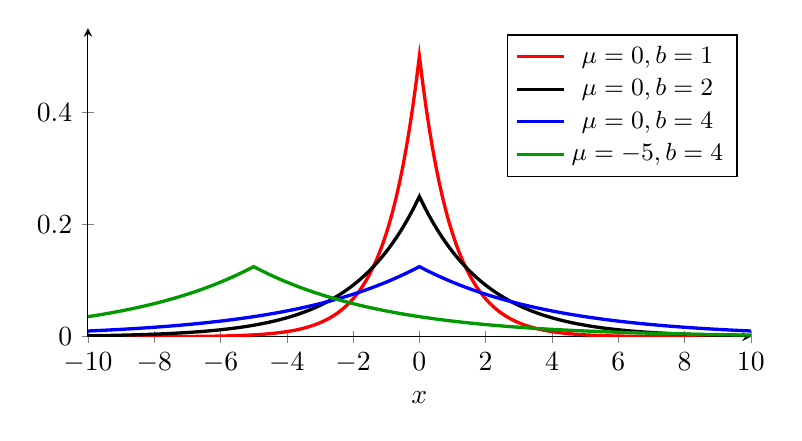
\begin{tikzpicture}
\begin{axis}[width=10cm,height=5.5cm,axis lines=left,xmin=-10,xmax=10,ymin=0,ymax=0.55,xlabel={$x$},samples=201,domain=-10:10,legend style={font=\small}]
\addplot[red,very thick] {0.5*exp(-abs(x))}; \addlegendentry{$\mu=0,b=1$}
\addplot[black,very thick] {0.25*exp(-abs(x)/2)}; \addlegendentry{$\mu=0,b=2$}
\addplot[blue,very thick] {0.125*exp(-abs(x)/4)}; \addlegendentry{$\mu=0,b=4$}
\addplot[green!60!black,very thick] {0.125*exp(-abs(x+5)/4)}; \addlegendentry{$\mu=-5,b=4$}
\end{axis}
\end{tikzpicture}
\end{center}

\subsection{توزیع بتا \lr{(Beta Distribution)}}
متغیر تصادفی بتا بین ۰ و ۱ تعریف شده و معمولاً برای مدل‌سازی احتمالاتی \textbf{خود احتمال وقوع یک پدیده} به کار می‌رود (مثلاً احتمال شیر آمدن یک سکه ناشناخته). این متغیر تصادفی دارای دو پارامتر آزاد $\alpha,\beta\in\R_{>0}$ است. به این پارامترها، پارامترهای شکلی (\lr{shape parameters}) نیز اطلاق می‌گردد. برای $X\sim\mathrm{Beta}(\alpha,\beta)$ در بازه $[0,1]$ یا $(0,1)$ (بسته به پارامترها):
\[
f_X(x)=\frac{\Gamma(\alpha+\beta)}{\Gamma(\alpha)\Gamma(\beta)}x^{\alpha-1}(1-x)^{\beta-1},
\]
که در آن $\Gamma(z)=\int_0^\infty t^{z-1}e^{-t}\dd t$ تابع گاما است (تعمیم فاکتوریل: $\Gamma(n)=(n-1)!$).

\begin{center}
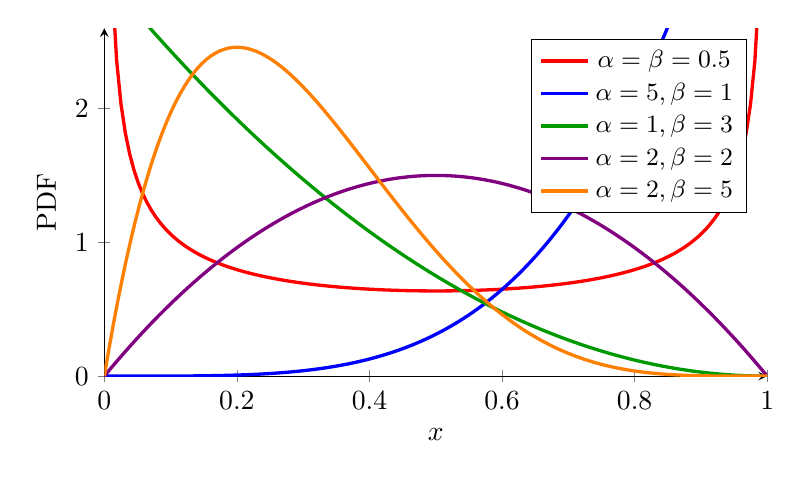
\begin{tikzpicture}
\begin{axis}[width=10cm,height=6cm,axis lines=left,xmin=0,xmax=1,ymin=0,ymax=2.6,xlabel={$x$},ylabel={\lr{PDF}},samples=150,legend style={font=\small},legend pos=north east]
\addplot[red,very thick,domain=0.012:0.988] {1/(pi*sqrt(x*(1-x)))}; \addlegendentry{$\alpha=\beta=0.5$}
\addplot[blue,very thick,domain=0:1] {5*x^4}; \addlegendentry{$\alpha=5,\beta=1$}
\addplot[green!60!black,very thick,domain=0:1] {3*(1-x)^2}; \addlegendentry{$\alpha=1,\beta=3$}
\addplot[violet,very thick,domain=0:1] {6*x*(1-x)}; \addlegendentry{$\alpha=2,\beta=2$}
\addplot[orange,very thick,domain=0:1] {30*x*(1-x)^4}; \addlegendentry{$\alpha=2,\beta=5$}
\end{axis}
\end{tikzpicture}
\end{center}

\begin{note}
\notetitle $\mathrm{Beta}(1,1)$ همان $\mathrm{Uniform}(0,1)$ است. منحنی $\alpha=\beta=0.5$ مثالی از چگالی است که در دو انتها به بی‌نهایت می‌رود (هرچند مساحت زیر آن ۱ است).
\end{note}

\subsection{برخی توزیع‌های کمتر کاربردی\ldots}
\begin{center}
\renewcommand{\arraystretch}{1.6}
\small
\begin{tabular}{c|c|c|c}
توزیع & پارامترها & تکیه‌گاه & \lr{PDF}\\\hline
رایلی \lr{(Rayleigh)} & $\sigma>0$ & $x\in[0,\infty)$ & $\dfrac{x}{\sigma^2}e^{-x^2/(2\sigma^2)}$\\
ارلانگ \lr{(Erlang)} & $k\in\{1,2,\ldots\},\ \lambda>0$ & $x\in[0,\infty)$ & $\dfrac{\lambda^kx^{k-1}e^{-\lambda x}}{(k-1)!}$\\
لاگ‌نرمال \lr{(Log-normal)} & $\mu\in\R,\ \sigma>0$ & $x\in(0,\infty)$ & $\dfrac{1}{x\sigma\sqrt{2\pi}}\exp\Big(-\dfrac{(\ln x-\mu)^2}{2\sigma^2}\Big)$
\end{tabular}
\end{center}
\begin{itemize}
\item \textbf{رایلی:} (با \lr{CDF} برابر $1-e^{-x^2/(2\sigma^2)}$) اندازه یک بردار دوبعدی با مؤلفه‌های گاوسی مستقل (مثلاً دامنه سیگنال در کانال‌های بی‌سیم با محوشدگی).
\item \textbf{ارلانگ:} زمان تا رخداد $k$ام در یک فرایند پواسون؛ مجموع $k$ متغیر نمایی مستقل. ($k=1$ همان نمایی است.)
\item \textbf{لاگ‌نرمال:} اگر $\ln X$ گاوسی باشد؛ برای کمیت‌هایی که حاصل‌ضرب عوامل تصادفی زیادند (مثل درآمد، اندازه فایل‌ها).
\end{itemize}

\section{تمرین‌های تکمیلی}

\begin{exercise}
فرض کنید $f_X(x)=cx^2$ برای $0\le x\le2$ و صفر در غیر این صورت. (الف) $c$ را بیابید. (ب) $F_X(x)$ را بیابید. (ج) $P(1<X\le2)$ را حساب کنید.
\end{exercise}
\begin{solution}
(الف) $\int_0^2cx^2\dd x=\frac{8c}{3}=1\Rightarrow c=\frac38$.
(ب) برای $0\le x\le2$: $F_X(x)=\int_0^x\frac38t^2\dd t=\frac{x^3}{8}$؛ برای $x<0$ صفر و برای $x>2$ یک.
(ج) $F_X(2)-F_X(1)=1-\frac18=\frac78$.
\end{solution}

\begin{exercise}
طول عمر یک هارد دیسک (بر حسب سال) نمایی با $\lambda=0.2$ است. (الف) احتمال اینکه بیش از ۵ سال کار کند چقدر است؟ (ب) اگر دیسکی ۳ سال کار کرده باشد، احتمال اینکه دست‌کم ۵ سال دیگر کار کند چقدر است؟ (ج) میانه طول عمر (عدد $m$ با $F(m)=\frac12$) را بیابید.
\end{exercise}
\begin{solution}
(الف) $P(X>5)=e^{-0.2\times5}=e^{-1}\approx0.368$.
(ب) با بی‌حافظگی: $P(X>8\given X>3)=P(X>5)\approx0.368$.
(ج) $1-e^{-0.2m}=\frac12\Rightarrow m=\frac{\ln2}{0.2}\approx3.47$ سال.
\end{solution}

\begin{exercise}
قد دانشجویان یک دانشگاه تقریباً $\mathcal N(170,10^2)$ (سانتی‌متر) است. چند درصد دانشجویان بین ۱۶۰ و ۱۹۰ سانتی‌متر قد دارند؟ (از $\Phi(1)\approx0.8413$ و $\Phi(2)\approx0.9772$ استفاده کنید.)
\end{exercise}
\begin{solution}
با استانداردسازی:
$P(160<X\le190)=\Phi\big(\frac{190-170}{10}\big)-\Phi\big(\frac{160-170}{10}\big)=\Phi(2)-\Phi(-1)=\Phi(2)-(1-\Phi(1))\approx0.9772-0.1587=0.8185$؛
یعنی حدود ۸۲٪.
\end{solution}

\begin{exercise}
متغیر $X$ با احتمال $\frac12$ برابر صفر است و با احتمال $\frac12$ از $\mathrm{Uniform}(0,1)$ پیروی می‌کند. \lr{CDF} آن را رسم کنید. آیا $X$ گسسته است یا پیوسته؟
\end{exercise}
\begin{solution}
برای $x<0$: $F=0$. برای $0\le x\le1$: $F(x)=\frac12+\frac12x$. برای $x>1$: $F=1$. \lr{CDF} در $x=0$ پرشی به اندازه $\frac12$ دارد و سپس به‌طور خطی تا ۱ بالا می‌رود. پس $X$ نه کاملاً گسسته است و نه کاملاً پیوسته؛ یک متغیر \textbf{ترکیبی} (\lr{mixed}) است. این مثال نشان می‌دهد چرا \lr{CDF} کلی‌ترین ابزار توصیف توزیع است (این متغیر \lr{PDF} معمولی ندارد).
\end{solution}
